\small

\noindent\fbox{\begin{minipage}{\dimexpr\textwidth-2\fboxsep-2\fboxrule\relax}
\begin{center}
\textbf{\textit{CELEBRAZIONI per il Santo NATALE - 2023}}
\end{center}
\end{minipage}}
\\

\noindent La Novena di Natale per giovani e adulti è da sabato 16 e fino al 23 dicembre. Da lunedì a venerdì alle ore 18.00, il sabato alle ore 18.30.

\noindent Il Triduo natalizio per i bambini sarà dal 21 al 23 alle ore 17.00.

\begin{tblr}{
      rows = {halign = c, valign = m},
      column{1} = {0.2\textwidth},
    }
% \toprule
Domenica 24 Dicembre
&
\makecell[c{p{0.7\textwidth}}]
{
Ore 8.00 e 10.30 SS. Messe festive. \\
Confessioni per tutto il giorno. \\
Ore 22.30, in chiesa il Coro S. Giorgio farà alcuni canti natalizi. \\
Ore 23.00, S. Messa nella Notte Santa.
}
\\
\hline
Lunedì 25 Dicembre
&
\makecell[c{p{0.7\textwidth}}]
{
Natale \\
Ore 8.00, 9.30, 11.00. SS. Messe. \\
Ore 16.00. Vesperi e Adorazione eucaristica.
}
\\
\hline
Martedì 26 Dicembre
&
\makecell[c{p{0.7\textwidth}}]
{
S. Stefano \\
Ore 9.00. S. Messa.
}
\\
\hline
Domenica 31 Dicembre
&
\makecell[c{p{0.7\textwidth}}]
{
Festa della Sacra Famiglia \\
Ore 18.30. S. Messa di fine anno col canto del Te Deum.
}
\\
\hline
Lunedì 1 Gennaio 2024
&
\makecell[c{p{0.7\textwidth}}]
{
Festa di Maria Madre di Dio. \\
Ricorre la Giornata Mondiale della Pace. \\
Ore 8.00, 10.30. SS. Messe. \\
Ore 16.00. Vesperi.
}
\\
\hline
Venerdì 5 Gennaio 2024
&
\makecell[c{p{0.7\textwidth}}]
{
Ore 18.30. Prefestiva dell’ Epifania.
}
\\
\hline
Sabato 6 Gennaio 2024
&
\makecell[c{p{0.7\textwidth}}]
{
Epifania \\
Festa dei santi Magi che adorano Gesù Bambino. \\
Ore 8.00, 10.30. SS. Messe. \\
Ore 16.00. Vesperi e conclusione col bacio a Gesù Bambino.
}
\\
\hline
Domenica 7 Gennaio 2024
&
\makecell[c{p{0.7\textwidth}}]
{
Festa del Battesimo di Gesù. \\
Ore 8.00, 10.30. SS. Messe.
}
\\
\hline
\end{tblr}


\begin{minipage}{0.25\textwidth}
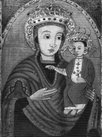
\includegraphics[width=\textwidth]{angolo.png}
\end{minipage}
\hfill
\begin{minipage}{0.65\textwidth}
Confessioni con preparazione comunitaria.

Per i giovanissimi e giovani a Maserada il giovedì 21 dicembre alle ore 20.30.

Per gli adulti a Breda martedì 19 dicembre ore 20.30 e a Candelù venerdì 22 dicembre ore 20.30.

A Maserada ci sarà un confessore straordinario oltre il parroco sabato 23 mattino e pomeriggio; la domenica 24 dalle 14.30 alle 18.00. Poi la chiesa viene chiusa fino alle ore 21.30.
\end{minipage}
\normalsize
